
% RUN:
% pdflatex -output-directory=/Users/salvatorpes/Desktop/Aprendizagem/Homework3/trash /Users/salvatorpes/Desktop/Aprendizagem/Homework3/G022.tex

% ir a settings.json e adicionar:
% // According to the wiki, the string latex-workshop.latex.autoBuild.run has three possible values: never, onSave and onFileChange(default).
% "latex-workshop.latex.autoBuild.run": "never",

\documentclass{article}


\author{Pedro Curvo (ist1102716) $|$ Salvador Torpes (ist1102474)}

\usepackage[utf8]{inputenc}
\usepackage[english]{babel}
% \usepackage[letterpaper,top=10mm,bottom=15mm,left=15mm,right=15mm,marginparwidth=1.75cm]{geometry}
% \usepackage[letterpaper,top=10mm,bottom=15mm,left=15mm,right=15mm,marginparwidth=1.75cm]{geometry}
\usepackage[letterpaper,margin=1in,marginparwidth=1.75cm]{geometry}
\usepackage{multicol}
\usepackage{biblatex}
\usepackage{cancel}
\usepackage{colortbl}
\addbibresource{Bibliografia.bib}
\usepackage{graphicx}
% \graphicspath{{../Homework1/images/}}
\usepackage{subcaption}
\usepackage{tabularx}
\usepackage{ulem}
\usepackage{booktabs}
\usepackage{array}
\usepackage{makecell}
\usepackage{multirow}
\usepackage{amsmath}
\usepackage{makecell}
\usepackage{url}
\usepackage{csquotes}
\usepackage{caption}
\usepackage{enumitem}
\usepackage{textcomp}
\usepackage{pdflscape}
\usepackage{makeidx}
\usepackage{amsmath}
% \usepackage{tocbibind}
\providecommand{\tightlist}{\relax}
\usepackage{tocloft}
\renewcommand{\cftsecindent}{0em}
\renewcommand{\cftsubsecindent}{1em}
\renewcommand{\cftsecfont}{\bfseries}
\renewcommand{\cftsubsecfont}{\itshape}
\setlength{\cftsubsecnumwidth}{0em}

\usepackage[version=4]{mhchem}
\usepackage{hyperref} % Remove "pdftex" option here
\usepackage{float}
\usepackage{fancyhdr}
\usepackage{ragged2e}
\usepackage{xkeyval}
%\usepackage{minted}
%\usemintedstyle{manni}
\usepackage{listings}
\usepackage{amssymb}




\usepackage{tikz}
\usetikzlibrary{positioning}
\usetikzlibrary{positioning, arrows.meta}
\usepackage{adjustbox}
\usepackage{sidecap}



% \usepackage[table,xcdraw]{xcolor}
\usepackage[LY1]{fontenc}
\usepackage{tikz-3dplot}
% \usepackage{pgfplots}
\usetikzlibrary{calc, 3d, arrows}
\usepackage{forest}




\usetikzlibrary{shapes.geometric, arrows}


\lstset{
    language=Python,
    basicstyle=\ttfamily,
    keywordstyle=\color{blue},
    commentstyle=\color{gray},
    stringstyle=\color{orange},
    numbers=left,
    numberstyle=\tiny,
    numbersep=5pt,
    showspaces=false,
    showstringspaces=false,
    breaklines=true,
    frame=tb,
    framexleftmargin=2em,
    xleftmargin=2em,
}


%\usepackage{fontspec}

%\setmonofont{Fira Code}

\fancyhf{}
\cfoot{\thepage}
\fancyhf{} % Clear all header and footer fields
\renewcommand{\headrulewidth}{0pt} % Remove the header rule line
\cfoot{\thepage} % Set the page number in the center of the footer

\pagestyle{fancy} % Apply the fancy page style

\setlength\columnsep{20pt}

\renewcommand{\familydefault}{\sfdefault}

\newenvironment{Figure}
  {\par\medskip\noindent\minipage{\linewidth}}
  {\endminipage\par\medskip}

\makeatletter
\newenvironment{figurehere}
{\def\@captype{figure}}
{}
\makeatother

\hypersetup{
  colorlinks,
  linkcolor=blue,
  anchorcolor=black,
  citecolor=cyan,
  filecolor=cyan,
  menucolor=cyan,
  urlcolor=cyan,
  bookmarksopen=true,
  bookmarksnumbered=true
}

\makeindex


\title{\vspace{-6mm}
\includegraphics[width=15mm,scale=2]{images/IST_Logo.png}\\ \vspace{5mm}
Machine Learning - Homework 3 \vspace{-5mm}}
\date{1st Term - 23/24}

\usepackage{sansmathfonts}
\usepackage[T1]{fontenc}
\usepackage[OT1]{fontenc}

\usepackage{listings}
\usepackage{xcolor}

\definecolor{codegreen}{rgb}{0,0.6,0}
\definecolor{codegray}{rgb}{0.5,0.5,0.5}
\definecolor{codepurple}{rgb}{0.58,0,0.82}
\definecolor{backcolour}{rgb}{0.95,0.95,0.92}

\lstdefinestyle{mystyle}{
  backgroundcolor=\color{backcolour},   
  commentstyle=\color{codegray},
  keywordstyle=\color{magenta},
  numberstyle=\tiny\color{codegray},
  stringstyle=\color{codegreen},
  keywordstyle=[2]{\color{orange}},
  keywords=[2]{plt.},
  basicstyle=\ttfamily\footnotesize,
  breakatwhitespace=false,         
  breaklines=true,                 
  captionpos=b,                    
  keepspaces=true,                 
  numbers=left,                    
  numbersep=5pt,                  
  showspaces=false,                
  showstringspaces=false,
  showtabs=false,                  
  tabsize=2,
  frame=single,
  framesep=2pt,
  framerule=0pt,
  xleftmargin=2pt,
  xrightmargin=2pt,
  aboveskip=1em,
  belowskip=1em,
  abovecaptionskip=0.5em,
  belowcaptionskip=0.5em,
  caption=\lstname,
  captionpos=b,
  language=Python,
  morekeywords={as},
  deletekeywords={None},
  emph={self},
  emphstyle=\color{blue},
  escapeinside={(*@}{@*)},
  literate={+}{{\textcolor{blue}{+}}}1
       {*}{{\textcolor{blue}{*}}}1
       {-}{{\textcolor{blue}{-}}}1
       {/}{{\textcolor{blue}{/}}}1
       {=}{{\textcolor{blue}{=}}}1
       {>}{{\textcolor{blue}{>}}}1
       {<}{{\textcolor{blue}{<}}}1
       {==}{{\textcolor{blue}{==}}}2
       {!=}{{\textcolor{blue}{!=}}}2
       {<=}{{\textcolor{blue}{<=}}}2
       {>=}{{\textcolor{blue}{>=}}}2,
  }
    
    \lstset{style=mystyle}
    \usepackage{fancyhdr}
    
    % Define header and footer styles
    \fancypagestyle{plain}{%
      \fancyhf{}% Clear header/footer
      \fancyhead[L]{Homework 3}% Header left
      \fancyhead[C]{2023/2024}% Header left
      \fancyhead[R]{Machine Learning}% Header right
      \fancyfoot[C]{\thepage}% Footer center
      \renewcommand{\headrulewidth}{0.4pt}% Header rule
      \renewcommand{\footrulewidth}{0pt}% Footer rule
    }
    
    % Apply the style to all pages except the first one
    \pagestyle{plain}
    \thispagestyle{empty} % Remove header/footer from first page


    \usepackage{amsmath} % for aligned
    %\usepackage{amssymb} % for \mathbb
    \usepackage{tikz}
    %\usepackage{etoolbox} % for \ifthen
    \usepackage{listofitems} % for \readlist to create arrays
    \usetikzlibrary{arrows.meta} % for arrow size
    \usepackage[outline]{contour} % glow around text
    \contourlength{1.4pt}
    
    \tikzset{>=latex} % for LaTeX arrow head
    \usepackage{xcolor}
    \colorlet{myred}{red!80!black}
    \colorlet{myblue}{blue!80!black}
    \colorlet{mygreen}{green!60!black}
    \colorlet{myyellow}{yellow!80!black}
    \colorlet{myorange}{orange!70!red!60!black}
    \colorlet{mydarkred}{red!30!black}
    \colorlet{mydarkblue}{blue!1!black}
    \colorlet{mydarkgreen}{green!30!black}
    \tikzstyle{node}=[thick,circle,draw=myblue,minimum size=22,inner sep=0.5,outer sep=0.6]
    \tikzstyle{node in}=[node,green!20!black,draw=mygreen!30!black,fill=myyellow!25]
    \tikzstyle{node hidden}=[node,blue!20!black,draw=myblue!30!black,fill=myorange!55]
    \tikzstyle{node convol}=[node,orange!20!black,draw=myorange!30!black,fill=myorange!20]
    \tikzstyle{node out}=[node,red!20!black,draw=myred!30!black,fill=myred!20]
    \tikzstyle{connect}=[thick,mydarkred] %,line cap=round
    \tikzstyle{connect arrow}=[-{Latex[length=4,width=3.5]},thick,mydarkblue,shorten <=0.5,shorten >=1]
    \tikzset{ % node styles, numbered for easy mapping with \nstyle
      node 1/.style={node in},
      node 2/.style={node hidden},
      node 3/.style={node out},
    }
    \def\nstyle{int(\lay<\Nnodlen?min(2,\lay):3)} % map layer number onto 1, 2, or 3


\begin{document}
    
\renewcommand{\arraystretch}{1.7}
\setlength{\columnseprule}{0.4pt}
\tdplotsetmaincoords{70}{110} % Set the viewing angle
\newcolumntype{M}[1]{>{\centering\arraybackslash\vspace{#1}}m{0.5\linewidth}<{\vspace{#1}}}
\newcolumntype{C}[2]{>{\centering\arraybackslash\vspace{#1}\rule{0pt}{#1}\hspace{0pt}}m{#2}}
\ifx\undefined\w
\newcolumntype{w}[1]{>{\centering\arraybackslash}m{#1}}
\fi
\renewcommand*\familydefault{\sfdefault} %% Only if the base font of the document is to be sans serif

% NEURAL NETWORK with coefficients, uniform arrows
\newcommand\setAngles[3]{
  \pgfmathanglebetweenpoints{\pgfpointanchor{#2}{center}}{\pgfpointanchor{#1}{center}}
  \pgfmathsetmacro\angmin{\pgfmathresult}
  \pgfmathanglebetweenpoints{\pgfpointanchor{#2}{center}}{\pgfpointanchor{#3}{center}}
  \pgfmathsetmacro\angmax{\pgfmathresult}
  \pgfmathsetmacro\dang{\angmax-\angmin}
  \pgfmathsetmacro\dang{\dang<0?\dang+360:\dang}
}

\maketitle
\vspace{-5mm}
\hrulefill




\section*{Pen and Paper Exercises}

\section*{1\textsuperscript{st} Question}

\subsection*{Dataset}

In this exercise we aim to learn a regression model for the following dataset:

\begin{table}[H]
    \centering
    \begin{tabular}{|c|c|c|c|c|}
        \hline
        Observation     & $x_0$ & $x_1$ & $x_2$ & output - $z$ \\ \hline
        $\vec{x}_1$               & 1     & 0.7   & -0.3  & 0.8           \\ \hline
        $\vec{x}_2$               & 1     & 0.4   & 0.5   & 0.6           \\ \hline
        $\vec{x}_3$               & 1     & -0.2  & 0.8   & 0.3           \\ \hline
        $\vec{x}_4$               & 1     & -0.4  & 0.3   & 0.3           \\ \hline
    \end{tabular}
    \caption{Dataset}
    \label{tab:my_label}
\end{table}

\[ X = \begin{bmatrix} 1 & 0.7 & -0.3 \\ 1 & 0.4 & 0.5 \\ 1 & -0.2 & 0.8 \\ 1 & -0.4 & 0.3 \end{bmatrix} \qquad Z = \begin{bmatrix} 0.8 \\ 0.6 \\ 0.3 \\ 0.3 \end{bmatrix} \]
\[ \vec{x}_1 = \begin{bmatrix} 0.7 \\ -0.3 \end{bmatrix} \qquad \vec{x}_2 = \begin{bmatrix} 0.4 \\ 0.5 \end{bmatrix} \qquad \vec{x}_3 = \begin{bmatrix} -0.2 \\ 0.8 \end{bmatrix} \qquad \vec{x}_4 = \begin{bmatrix} -0.4 \\ 0.3 \end{bmatrix} \]

\subsection*{a)}

\subsubsection*{Transforming the data}

We are transforming our original data into a new space, according to the radial basis function:

\[ \phi_j(\vec{x}) = \exp \left( - \frac{||\vec{x} - c_j||^2}{2} \right) \]

\[ c_1 = \begin{bmatrix} 0 \\ 0 \end{bmatrix} \qquad c_2 = \begin{bmatrix} 1 \\ -1 \end{bmatrix} \qquad c_3 = \begin{bmatrix} -1 \\ 1 \end{bmatrix} \]

After applying the transformation, we will have 3 new inputs for each observation. Therefore, the new dataset will look like:

\[ \Phi(X) =  X_{trans} = \begin{bmatrix} 1 & \phi_1(\vec{x}_1) & \phi_2(\vec{x}_1) & \phi_3(\vec{x}_1) \\ 1 & \phi_1(\vec{x}_2) & \phi_2(\vec{x}_2) & \phi_3(\vec{x}_2) \\ 1 & \phi_1(\vec{x}_3) & \phi_2(\vec{x}_3) & \phi_3(\vec{x}_3) \\ 1 & \phi_1(\vec{x}_4) & \phi_2(\vec{x}_4) & \phi_3(\vec{x}_4) \end{bmatrix} \]

\paragraph{Observation 1}

If we apply our transformation to the first observation $\vec{x}_1$, we get:

\[ \phi_1(\vec{x}_1) = \exp \left( - \frac{||\vec{x}_1 - c_1||^2}{2} \right) = \exp \left( - \frac{0.58}{2} \right) = 0.74826 \]

\[ \phi_2(\vec{x}_1) = \exp \left( - \frac{||\vec{x}_1 - c_2||^2}{2} \right) = \exp \left( - \frac{0.58}{2} \right) = 0.74826 \]

\[ \phi_3(\vec{x}_1) = \exp \left( - \frac{||\vec{x}_1 - c_3||^2}{2} \right) = \exp \left( - \frac{4.58}{2} \right) = 0.10127 \]

\paragraph{Observation 2}

If we apply our transformation to the second observation $\vec{x}_2$, we get:

\[ \phi_1(\vec{x}_2) = \exp \left( - \frac{||\vec{x}_2 - c_1||^2}{2} \right) = \exp \left( - \frac{0.41}{2} \right) = 0.81465 \]

\[ \phi_2(\vec{x}_2) = \exp \left( - \frac{||\vec{x}_2 - c_2||^2}{2} \right) = \exp \left( - \frac{2.61}{2} \right) = 0.27117 \]

\[ \phi_3(\vec{x}_2) = \exp \left( - \frac{||\vec{x}_2 - c_3||^2}{2} \right) = \exp \left( - \frac{2.21}{2} \right) = 0.33121 \]

\paragraph{Observation 3}

If we apply our transformation to the third observation $\vec{x}_3$, we get:

\[ \phi_1(\vec{x}_3) = \exp \left( - \frac{||\vec{x}_3 - c_1||^2}{2} \right) = \exp \left( - \frac{0.68}{2} \right) = 0.71177 \]

\[ \phi_2(\vec{x}_3) = \exp \left( - \frac{||\vec{x}_3 - c_2||^2}{2} \right) = \exp \left( - \frac{4.68}{2} \right) = 0.09633 \]

\[ \phi_3(\vec{x}_3) = \exp \left( - \frac{||\vec{x}_3 - c_3||^2}{2} \right) = \exp \left( - \frac{0.68}{2} \right) = 0.71177 \]

\paragraph{Observation 4}

If we apply our transformation to the fourth observation $\vec{x}_4$, we get:

\[ \phi_1(\vec{x}_4) = \exp \left( - \frac{||\vec{x}_4 - c_1||^2}{2} \right) = \exp \left( - \frac{0.25}{2} \right) = 0.88250 \]

\[ \phi_2(\vec{x}_4) = \exp \left( - \frac{||\vec{x}_4 - c_2||^2}{2} \right) = \exp \left( - \frac{3.65}{2} \right) = 0.16122 \]

\[ \phi_3(\vec{x}_4) = \exp \left( - \frac{||\vec{x}_4 - c_3||^2}{2} \right) = \exp \left( - \frac{0.85}{2} \right) = 0.65377 \]

\subsubsection*{Transformed Dataset}

After applying the transformation, we get the following dataset:

\[ \Phi(X) = X_{trans} = \begin{bmatrix}
    1 & 0.74826 & 0.74826 & 0.10127 \\
    1 & 0.81465 & 0.27117 & 0.33121 \\
    1 & 0.71177 & 0.09633 & 0.71177 \\
    1 & 0.88250 & 0.16122 & 0.65377
\end{bmatrix} \]

\begin{table}[H]
    \centering
    \begin{tabular}{|c|c|c|c|c|c|}
        \hline
        Observation     & $\phi_0$ & $\phi_1$ & $\phi_2$ & $\phi_3$ & output - $z$ \\ \hline
        $\vec{x}_1$               & 1     & 0.74826   & 0.74826  & 0.10127 & 0.8           \\ \hline
        $\vec{x}_2$               & 1     & 0.81465   & 0.27117   & 0.33121  & 0.6           \\ \hline
        $\vec{x}_3$               & 1     & 0.71177  & 0.09633   & 0.71177   & 0.3           \\ \hline
        $\vec{x}_4$               & 1     & 0.88250  & 0.16122   & 0.65377   & 0.3           \\ \hline
    \end{tabular}
    \caption{Transformed Dataset}
    \label{tab:my_label}
\end{table}

\subsubsection*{Ridge Regression}

A regression model is characterized by a column matrix of weights $W$ - if we multiply $W$ by a new observation, we get the estimated output for that observation.

\[ \hat{z} = w_0 + \sum_{j=1}^{M} w_j x_j = X \cdot W \]

$X$ is the matrix of observations, and $W$ is the matrix of weights:

\[ X = \begin{bmatrix} 1 & \vec{x}_1^T \\ 1 & \vec{x}_2^T \\ 1 & \vec{x}_3^T \\ 1 & \vec{x}_4^T \end{bmatrix} \qquad W = \begin{bmatrix} w_0 \\ w_1 \\ w_2 \\ w_3 \end{bmatrix} \]

When considering the case where we \textbf{transform} our data according to a function $\phi$, the regression formula is:

\[ \hat{z} = w_0 + \sum_{j=1}^{M} w_j \phi_j(x) = \Phi(X) \cdot W \]

The Ridge Regression ($l_2$ regularization) is a method that penalizes the weights of the model, in order to avoid overfitting. The formula for $W$ matrix in the Ridge Regression is:

\[ W = ( \Phi^T \Phi + \lambda I )^{-1} \Phi^T Z \]

Where $\lambda$ is the regularization parameter ($\lambda = 0.1$), $I$ is the identity matrix and $\Phi$ is the matrix of transformed observations.

\subsubsection*{Computing the weights}

Using the formula for $W$, we get:

\[ 
    \Phi = \begin{bmatrix}
    1 & 0.74826 & 0.74826 & 0.10127 \\
    1 & 0.81465 & 0.27117 & 0.33121 \\
    1 & 0.71177 & 0.09633 & 0.71177 \\
    1 & 0.88250 & 0.16122 & 0.65377
\end{bmatrix} 
\qquad 
Z = \begin{bmatrix} 0.8 \\ 0.6 \\ 0.3 \\ 0.3 \end{bmatrix} \
\qquad 
\Phi^T = \begin{bmatrix}
    1 & 1 & 1 & 1 \\
    0.74826 & 0.81465 & 0.71177 & 0.88250 \\
    0.74826 & 0.27117 & 0.09633 & 0.16122 \\
    0.10127 & 0.33121 & 0.71177 & 0.65377
\end{bmatrix} \]

\[ (\Phi^T \Phi - \lambda I)^{-1} = \begin{bmatrix}
    4.54826  & -3.77682 & -1.86117 & -1.86155 \\
    -3.77682 & 5.98285  & -0.88543 & -1.26432 \\
    -1.86117 & -0.88543 &  4.33276 &  2.72156 \\
    -1.86155 & -1.26432 &  2.72156 &  4.53204 \\
\end{bmatrix} \]

\[ W = (\Phi^T \Phi + \lambda I)^{-1} \Phi^T Z = \begin{bmatrix} w_0 \\ w_1 \\ w_2 \\ w_3 \end{bmatrix} = \begin{bmatrix} 0.33914 \\ 0.19945 \\ 0.40096 \\ -0.29600 \end{bmatrix} \]

\subsubsection*{Final form of the prediction function}

In order to compute $\hat{z}$, we need to multiply the weights by the transformed observation:

\[ \hat{z} = \sum_{j=0}^{3} w_j \phi_j(x) = \Phi(X) \cdot W  \Leftrightarrow \]
\[ \Leftrightarrow \hat{z} = w_0 + w_1 \cdot \phi_1 + w_2 \cdot \phi_2 + w_3 \cdot \phi_3 = 0.33914 + 0.19945 \cdot \phi_1 + 0.40096 \cdot \phi_2 - 0.29600 \cdot \phi_3 \]

\paragraph{}
Using our dataset, the predicted values are:

\[ \hat{z} = \begin{bmatrix}
    0.75844 \\
    0.51232 \\
    0.30905 \\
    0.38629
\end{bmatrix} \]

\subsection*{b)}

The RMSE (Root Mean Squared Error) is a metric that measures the difference between the predicted values and the actual values. It is defined as:

\[ RMSE = \sqrt{\frac{1}{N} \sum_{i=1}^{N} (z_i - \hat{z}_i)^2} \]

Where $z_i$ is the actual value and $\hat{z}_i$ is the predicted value.
In our case, we have the following data:

\begin{table}[H]
    \centering
    \begin{tabular}{|c|c|}
        \hline
        $z_i$ & $\hat{z}_i$ \\ \hline
        0.8   & 0.75844     \\ \hline
        0.6   & 0.51232     \\ \hline
        0.3   & 0.30905     \\ \hline
        0.3   & 0.38629     \\ \hline
    \end{tabular}
    \caption{Actual and Predicted Values}
    \label{tab:my_label}
\end{table}

The RMSE is:

\[ RMSE = \sqrt{\frac{1}{4} \sum_{i=1}^{4} (z_i - \hat{z}_i)^2} = \sqrt{\frac{1}{4} \cdot 0.01694} = 0.06508 \]


\newpage

\section*{2\textsuperscript{nd} Question}

\subsection*{Structure of the Network}

We are considering a MLP (Multi-Layer Perceptron) with 2 hidden layers. The input and output layers have 4 and 3 nodes, respectively. This means we have 4 input features and 3 output features. 
Our structure is the following:

\begin{center}
% NEURAL NETWORK with coefficients, no arrows
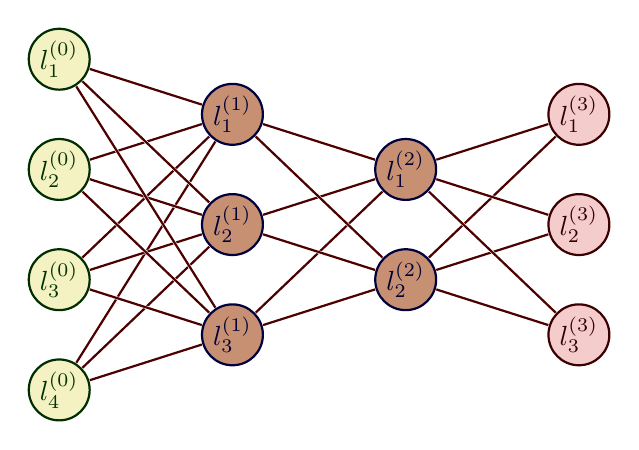
\begin{tikzpicture}[x=2.2cm,y=1.4cm]
\message{^^JNeural network without arrows}
\readlist\Nnod{4,3,2,3} % array of number of nodes per layer

\message{^^J  Layer}
\foreachitem \N \in \Nnod{ % loop over layers
    \def\lay{\Ncnt} % alias of index of current layer
    \pgfmathsetmacro\prev{int(\Ncnt-1)} % number of previous layer
    \message{\lay,}
    \foreach \i [evaluate={\y=\N/2-\i; \x=\lay; \n=\nstyle;}] in {1,...,\N}{ % loop over nodes
    
    % NODES
    \node[node \n] (N\lay-\i) at (\x,\y) {$l_\i^{(\prev)}$};
    
    % CONNECTIONS
    \ifnum\lay>1 % connect to previous layer
        \foreach \j in {1,...,\Nnod[\prev]}{ % loop over nodes in previous layer
        \draw[connect,white,line width=1.2] (N\prev-\j) -- (N\lay-\i);
        \draw[connect] (N\prev-\j) -- (N\lay-\i);
        %\draw[connect] (N\prev-\j.0) -- (N\lay-\i.180); % connect to left
        }
    \fi % else: nothing to connect first layer
    
    }
}

% LABELS
% \node[above=5,align=center,mygreen!60!black] at (N1-1.90) {input\\[-0.2em]layer};
% \node[above=2,align=center,myblue!60!black] at (N3-1.90) {hidden layer};
% \node[above=8,align=center,myred!60!black] at (N\Nnodlen-1.90) {output\\[-0.2em]layer};

\end{tikzpicture}
\end{center}

\subsection*{Activation Function}

The activation function is the hyperbolic tangent function and it is the same for all layers:

\[ \Phi(x) = f(x) = \tanh(0.5x-2) \]

\[ \Phi'(x) = f'(x) = \frac{0.5}{\cosh^2(0.5x-2)} =0.5 \cdot \left( 1 - \tanh^2(0.5x-2) \right) = 0.5 \cdot \left( 1 - \Phi^2(x) \right) \]

\subsection*{Loss Function}

The loss function is the mean square error:

\[ E(W) = \frac{1}{2} \sum_{i=1}^{N} ||z_i - \hat{z}_i||^2 \]

\subsection*{Initial Weights}

We are told the initial weights are:

\[ w^{[1]} = \begin{bmatrix} 1 & 1 & 1 & 1 \\ 1 & 1 & 2 & 1 \\ 1 & 1 & 1 & 1 \end{bmatrix} \qquad w^{[2]} = \begin{bmatrix} 1 & 4 & 1 \\ 1 & 1 & 1 \end{bmatrix} \qquad w^{[3]} = \begin{bmatrix} 1 & 1  \\ 3 & 1 \\ 1 & 1 \end{bmatrix} \]
\[ b^{[1]} = \begin{bmatrix} 1 \\ 1 \\ 1 \end{bmatrix} \qquad b^{[2]} = \begin{bmatrix} 1 \\ 1 \end{bmatrix} \qquad b^{[3]} = \begin{bmatrix} 1 \\ 1 \\ 1 \end{bmatrix} \]

\subsection*{Forward Propagation}

According to these weights, we can compute the initial values for $X^{[1]}$, $X^{[2]}$ and $X^{[3]}$. 
We are considering two training observations and therefore have two different $X^{[0]}$ vectors:

\[ X^{[0]}_1 = \begin{bmatrix} 1 \\ 1 \\ 1 \\ 1  \end{bmatrix} \qquad X^{[0]}_2 = \begin{bmatrix} 1 \\ 0 \\ 0 \\ -1  \end{bmatrix} \]

With $X^{[0]}$ we can compute $X^{[1]}$, $X^{[2]}$ and $X^{[3]}$ - Propagation of both inputs through the network:

\[ X^{[1]}_1 = \Phi(W^{[1]} \cdot X^{[0]}_1 + b^{[1]}) = \tanh \left( \left(\begin{bmatrix} 1 & 1 & 1 & 1 \\ 1 & 1 & 2 & 1 \\ 1 & 1 & 1 & 1 \end{bmatrix} \cdot \begin{bmatrix} 1 \\ 1 \\ 1 \\ 1 \end{bmatrix} + \begin{bmatrix} 1 \\ 1 \\ 1 \end{bmatrix} \right) \cdot 0.5 - 2I \right) = \tanh \left( \begin{bmatrix} 0.5 \\ 1 \\ 0.5 \end{bmatrix} \right)  = \begin{bmatrix} 0.46212 \\ 0.76159 \\ 0.46212 \end{bmatrix} \]

\[ Z^{[1]}_1 = W^{[1]} \cdot X^{[0]}_1 + b^{[1]} = \begin{bmatrix} 5 \\ 6 \\ 5 \end{bmatrix} \]

\[ X^{[2]}_1 = \Phi(W^{[2]} \cdot X^{[1]}_1 + b^{[2]}) = \tanh \left( \left(\begin{bmatrix} 1 & 4 & 1 \\ 1 & 1 & 1 \end{bmatrix} \cdot \begin{bmatrix} 0.46212 \\ 0.76159 \\ 0.46212 \end{bmatrix} + \begin{bmatrix} 1 \\ 1 \end{bmatrix} \right) \cdot 0.5 - 2I \right) = \tanh \left( \begin{bmatrix} 0.45048 \\ -0.57642 \end{bmatrix} \right)  = \begin{bmatrix} 0.45048 \\ -0.57642 \end{bmatrix} \]

\[ Z^{[2]}_1 = W^{[2]} \cdot X^{[1]}_1 + b^{[2]} = \begin{bmatrix} 4.97061 \\ 2.68583 \end{bmatrix} \]

\[ X^{[3]}_1 = \Phi(W^{[3]} \cdot X^{[2]}_1 + b^{[3]}) = \tanh \left( \left(\begin{bmatrix} 1 & 1  \\ 3 & 1 \\ 1 & 1 \end{bmatrix} \cdot \begin{bmatrix} 0.45048 \\ -0.57642 \end{bmatrix} + \begin{bmatrix} 1 \\ 1 \\ 1 \end{bmatrix} \right) \cdot 0.5 - 2I \right) = \tanh \left( \begin{bmatrix} -1.56297 \\ -1.11249 \\ -1.56297 \end{bmatrix} \right)  = \begin{bmatrix} -0.9159 \\ -0.80494 \\ -0.9159 \end{bmatrix} \]

\[ Z^{[3]}_1 = W^{[3]} \cdot X^{[2]}_1 + b^{[3]} = \begin{bmatrix} 0.87406 \\ 1.77503 \\ 0.87406 \end{bmatrix} \]

\[ X^{[1]}_2 = \Phi(W^{[1]} \cdot X^{[0]}_2 + b^{[1]}) = \tanh \left( \left(\begin{bmatrix} 1 & 1 & 1 & 1 \\ 1 & 1 & 2 & 1 \\ 1 & 1 & 1 & 1 \end{bmatrix} \cdot \begin{bmatrix} 1 \\ 0 \\ 0 \\ -1 \end{bmatrix} + \begin{bmatrix} 1 \\ 1 \\ 1 \end{bmatrix} \right) \cdot 0.5 - 2I \right) = \tanh \left( \begin{bmatrix} -1.5 \\ -1.5 \\ -1.5 \end{bmatrix} \right)  = \begin{bmatrix} -0.90515 \\ -0.90515 \\ -0.90515 \end{bmatrix} \]

\[ Z^{[1]}_2 = W^{[1]} \cdot X^{[0]}_2 + b^{[1]} = \begin{bmatrix} 1 \\ 1 \\ 1 \end{bmatrix} \]

\[ X^{[2]}_2 = \Phi(W^{[2]} \cdot X^{[1]}_2 + b^{[2]}) = \tanh \left( \left(\begin{bmatrix} 1 & 4 & 1 \\ 1 & 1 & 1 \end{bmatrix} \cdot \begin{bmatrix} -0.90515 \\ -0.90515 \\ -0.90515 \end{bmatrix} + \begin{bmatrix} 1 \\ 1 \end{bmatrix} \right) \cdot 0.5 - 2I \right) = \tanh \left( \begin{bmatrix} -4.21544 \\ -2.85772 \end{bmatrix} \right)  = \begin{bmatrix} -0.99956 \\ -0.99343 \end{bmatrix} \]

\[ Z^{[2]}_2 = W^{[2]} \cdot X^{[1]}_2 + b^{[2]} = \begin{bmatrix} -4.43089 \\ -1.71544 \end{bmatrix} \]

\[ X^{[3]}_2 = \Phi(W^{[3]} \cdot X^{[2]}_2 + b^{[3]}) = \tanh \left( \left(\begin{bmatrix} 1 & 1  \\ 3 & 1 \\ 1 & 1 \end{bmatrix} \cdot \begin{bmatrix} -0.99956 \\ -0.99343 \end{bmatrix} + \begin{bmatrix} 1 \\ 1 \\ 1 \end{bmatrix} \right) \cdot 0.5 - 2I \right) = \tanh \left( \begin{bmatrix} -2.4965 \\ -3.49606 \\ -2.4965 \end{bmatrix} \right)  = \begin{bmatrix} -0.98652 \\ -0.99816 \\ -0.98652 \end{bmatrix} \]

\[ Z^{[3]}_2 = W^{[3]} \cdot X^{[2]}_2 + b^{[3]} = \begin{bmatrix} -0.993 \\ -2.99212 \\ -0.993 \end{bmatrix} \]

\subsection*{Output Values}

Since we ate working with a activation function whose range is $[-1, 1]$, the output values for both observations are:

\[ t_1 = \begin{bmatrix} -1 \\ 1 \\ -1 \end{bmatrix} \qquad t_2 = \begin{bmatrix} 1 \\ -1 \\ -1 \end{bmatrix} \]

\subsection*{Gradient Descent}

According to the gradient descent formula, in order to update the weights we need to compute the gradient of the loss function with respect to the weights.
We are considering the following loss function for each observation:

\[ E(W) = \frac{1}{2} || z-\hat{z} ||^2 = \frac{1}{2} (z-\hat{z})^2 = \frac{1}{2} (X^{[P]} - t)^2 \]


Where $z = t$ is vector of actual output values for the observation and $\hat{z} = X^{[P]}$ ($P$ is the index of the last layer) is the vector of predicted output values for the observation. 
When doing the gradient descent, we need to compute the updated weights for each layer of the network.
The updated weight is equal to:

\begin{align*}
    W^{[p]}_{\text{new}} = W^{[p]} - \eta &\frac{\partial E(W)}{\partial W^{[p]}} \\
    &\frac{\partial E(W)}{\partial W^{[P]}} = \delta^{[P]} \cdot \frac{\partial Z^{[P]}}{\partial W^{[P]}} = \delta^{[P]} \cdot (X^{[P-1]})^T  \text{,      if } p = P \text{ (output layer)} \\
    &\frac{\partial E(W)}{\partial W^{[p]}} = \delta^{[p]} \cdot \frac{\partial Z^{[p]}}{\partial W^{[p]}} = \delta^{[p]} \cdot (X^{[p-1]})^T  \text{,      if } p \neq P \text{ (hidden layer)} \\
\end{align*}

We can compute $\delta^{[p]}$ and $\delta^{[P]}$ as:

\begin{align*}
    &\delta^{[P]} = \frac{\partial E(W)}{\partial Z^{[P]}} = \frac{\partial E(W)}{\partial X^{[P]}} \circ \frac{\partial X^{[P]}}{\partial Z^{[P]}} = (X^{[P]}-t) \circ \Phi'^{[P]}(Z^{[P]}) \\
    &\delta^{[p]} = \frac{\partial E(W)}{\partial Z^{[p]}} = \left( \frac{\partial Z^{[p+1]}}{\partial X^{[p]}} \right)^T \cdot \delta^{[p+1]} \circ \frac{\partial X^{[p]}}{\partial Z^{[p]}} = (W^{[p+1]})^T \cdot \delta^{[p+1]} \circ \Phi'^{[p]}(Z^{[p]}) \\
\end{align*}

We also need to update the biases, according to the following formula:

\begin{align*}
    b^{[p]}_{\text{new}} = b^{[p]} - \eta &\frac{\partial E(W)}{\partial b^{[p]}} \\
    &\frac{\partial E(W)}{\partial b^{[p]}} = \delta^{[p]} \cdot \frac{\partial Z^{[p]}}{\partial b^{[p]}} = \delta^{[p]} \\
\end{align*}

Therefore, we can write:

\[ b^{[p]}_{\text{new}} = b^{[p]} - \eta\delta^{[p]} \]

\subsection*{Computing the updated weights}

We are performing a batch gradient descent, therefore, the updated weight will be computed using the gradients of all observations (2 in our case):

\[ W^{[n]}_{\text{new}} = W^{[n]} +\Delta W^{[n]} = W^{[n]} - \eta \sum_i \frac{\partial E(W)}{\partial W^{[n]}_i} \]

Where $i$ is the index of the observation.

\subsubsection*{Updating $W^{[3]}$}

The weight variation of $W^{[3]}$ coming from the first observation is:

\begin{align*}
    \Delta W^{[3]}_1 &= - \eta \frac{\partial E(W)}{\partial W^{[3]}_1} = \\
    &= - \eta \cdot (X^{[3]}_1 - t_1) \circ \Phi'^{[3]}(Z^{[3]}_1)\cdot (X^{[2]}_1)^T =\\
    &= - 0.1 \cdot 0.5 \cdot (X^{[3]}_1 - t_1)  \circ \left( 1 - \tanh^2(Z^{[3]}_1 \cdot 0.5 - 2) \right) \cdot (X^{[2]}_1)^T = \\
    &= \begin{bmatrix} -0.00031 &  0.00039 \\   0.01431 & -0.01831 \\  -0.00031 &  0.00039  \end{bmatrix} \\
\end{align*}

The weight variation of $W^{[3]}$ coming from the second observation is:

\begin{align*}
    \Delta W^{[3]}_2 &= - \eta \frac{\partial E(W)}{\partial W^{[3]}_2} = \\
    &= - \eta \cdot (X^{[3]}_2 - t_2) \circ \Phi'^{[3]}(Z^{[3]}_2)\cdot (X^{[2]}_2)^T =\\
    &= - 0.1 \cdot 0.5 \cdot (X^{[3]}_2 - t_2)  \circ \left( 1 - \tanh^2(Z^{[3]}_2 \cdot 0.5 - 2) \right) \cdot (X^{[2]}_2)^T = \\
    &= \begin{bmatrix} -2.65845\times 10^{-3} & -2.64215\times 10^{-3} \\   3.40000\times 10^{-7} &  3.30000\times 10^{-7} \\   1.80400\times 10^{-5} &  1.79300\times 10^{-5}  \end{bmatrix} \\
\end{align*}

The total weight variation of $W^{[3]}$ is:

\[ \Delta W^{[3]} = \Delta W^{[3]}_1 + \Delta W^{[3]}_2 =  \begin{bmatrix} -0.00296 & -0.00225 \\   0.01431 & -0.01831 \\  -0.00029 &  0.00041  \end{bmatrix} \]

The updated weight $W^{[3]}$ is:

\[ W^{[3]}_{\text{new}} = W^{[3]} + \Delta W^{[3]} = \begin{bmatrix} 0.99704 & 0.99775 \\  3.01431 & 0.98169 \\  0.99971 & 1.00041  \end{bmatrix} \]

\subsubsection*{Updating $W^{[2]}$}

\paragraph{} The weight variation of $W^{[2]}$ coming from the first observation is:

\begin{align*}
    \Delta W^{[2]}_1 &= - \eta \frac{\partial E(W)}{\partial W^{[2]}_1} = - \eta \cdot (W^{[3]}_1)^T \cdot \delta^{[3]}_1 \circ \Phi'^{[2]}(Z^{[2]}_1)\cdot (X^{[1]}_1)^T = \\
    &= - \eta \cdot (W^{[3]}_1)^T \cdot \left( (X^{[3]}_1 - t_1) \circ \Phi'^{[3]}(Z^{[3]}_1) \right) \circ \Phi'^{[2]}(Z^{[2]}_1) \cdot (X^{[1]}_1)^T = \\
    &= -0.1 \cdot 0.5 \cdot 0.5 \cdot (W^{[3]}_1)^T \cdot \left( (X^{[3]}_1 - t_1) \circ \left( 1 - \tanh^2(Z^{[3]}_1 \cdot 0.5 - 2) \right) \right) \circ \left( 1 - \tanh^2(Z^{[2]}_1 \cdot 0.5 - 2) \right) \cdot (X^{[1]}_1)^T = \\
    &= \begin{bmatrix} 0.01731 & 0.02852 & 0.01731 \\  0.00469 & 0.00773 & 0.00469  \end{bmatrix} \\
\end{align*}

The weight variation of $W^{[2]}$ coming from the second observation is:

\begin{align*}
    \Delta W^{[2]}_2 &= - \eta \frac{\partial E(W)}{\partial W^{[2]}_2} = - \eta \cdot (W^{[3]}_2)^T \cdot \delta^{[3]}_2 \circ \Phi'^{[2]}(Z^{[2]}_2)\cdot (X^{[1]}_2)^T = \\
    &= - \eta \cdot (W^{[3]}_2)^T \cdot \left( (X^{[3]}_2 - t_2) \circ \Phi'^{[3]}(Z^{[3]}_2) \right) \circ \Phi'^{[2]}(Z^{[2]}_2) \cdot (X^{[1]}_2)^T = \\
    &= -0.1 \cdot 0.5 \cdot 0.5 \cdot (W^{[3]}_2)^T \cdot \left( (X^{[3]}_2 - t_2) \circ \left( 1 - \tanh^2(Z^{[3]}_2 \cdot 0.5 - 2) \right) \right) \circ \left( 1 - \tanh^2(Z^{[2]}_2 \cdot 0.5 - 2) \right) \cdot (X^{[1]}_2)^T = \\
    &= \begin{bmatrix} -1.04180\times 10^{-6} & -1.04180\times 10^{-6} & -1.04180\times 10^{-6} \\  -1.56499\times 10^{-5} & -1.56499\times 10^{-5} & -1.56499\times 10^{-5}  \end{bmatrix} \\
\end{align*}

The total weight variation of $W^{[2]}$ is:

\[ \Delta W^{[2]} = \Delta W^{[2]}_1 + \Delta W^{[2]}_2 = \begin{bmatrix} 0.0173  & 0.02852 & 0.0173  \\  0.00468 & 0.00772 & 0.00468  \end{bmatrix}  \]

The updated weight $W^{[2]}$ is:

\[ W^{[2]}_{\text{new}} = W^{[2]} + \Delta W^{[2]} = \begin{bmatrix} 1.0173  & 4.02852 & 1.0173  \\  1.00468 & 1.00772 & 1.00468  \end{bmatrix} \]

\subsubsection*{Updating $W^{[1]}$}

The weight variation of $W^{[1]}$ coming from the first observation is:

\begin{align*}
     \Delta W^{[1]}_1 &= - \eta \frac{\partial E(W)}{\partial W^{[1]}_1} = - \eta \cdot (W^{[2]}_1)^T \cdot \delta^{[2]}_1 \circ \Phi'^{[1]}(Z^{[1]}_1)\cdot (X^{[0]}_1)^T = \\
    &= - \eta \cdot (W^{[2]}_1)^T \cdot \left( (W^{[3]}_1)^T \cdot \delta^{[3]}_1 \circ \Phi'^{[2]}(Z^{[2]}_1) \right) \circ \Phi'^{[1]}(Z^{[1]}_1) \cdot (X^{[0]}_1)^T = \\
    &= - \eta \cdot (W^{[2]}_1)^T \cdot \left( (W^{[3]}_1)^T \cdot \left( (X^{[3]}_1 - t_1) \circ \Phi'^{[3]}(Z^{[3]}_1) \right) \circ \Phi'^{[2]}(Z^{[2]}_1) \right) \circ \Phi'^{[1]}(Z^{[1]}_1) \cdot (X^{[0]}_1)^T = \\
    &= -0.1 \cdot 0.5 \cdot 0.5 \cdot 0.5 \cdot (W^{[2]}_1)^T \cdot \left( (W^{[3]}_1)^T \cdot \left( (X^{[3]}_1 - t_1) \circ \left( 1 - \tanh^2(Z^{[3]}_1 \cdot 0.5 - 2) \right) \right) \circ \left( 1 - \tanh^2(Z^{[2]}_1 \cdot 0.5 - 2) \right) \right) \circ \\
    &\circ \left( 1 - \tanh^2(Z^{[1]}_1 \cdot 0.5 - 2) \right) \cdot (X^{[0]}_1)^T = \\
    &=  \begin{bmatrix} 0.01872 & 0.01872 & 0.01872 & 0.01872 \\  0.03359 & 0.03359 & 0.03359 & 0.03359 \\  0.01872 & 0.01872 & 0.01872 & 0.01872  \end{bmatrix}
\end{align*}

The weight variation of $W^{[1]}$ coming from the second observation is:

\begin{align*}
    \Delta W^{[1]}_2 &= - \eta \frac{\partial E(W)}{\partial W^{[1]}_2} = - \eta \cdot (W^{[2]}_2)^T \cdot \delta^{[2]}_2 \circ \Phi'^{[1]}(Z^{[1]}_2)\cdot (X^{[0]}_2)^T = \\
    &= - \eta \cdot (W^{[2]}_2)^T \cdot \left( (W^{[3]}_2)^T \cdot \delta^{[3]}_2 \circ \Phi'^{[2]}(Z^{[2]}_2) \right) \circ \Phi'^{[1]}(Z^{[1]}_2) \cdot (X^{[0]}_2)^T = \\
    &= - \eta \cdot (W^{[2]}_2)^T \cdot \left( (W^{[3]}_2)^T \cdot \left( (X^{[3]}_2 - t_2) \circ \Phi'^{[3]}(Z^{[3]}_2) \right) \circ \Phi'^{[2]}(Z^{[2]}_2) \right) \circ \Phi'^{[1]}(Z^{[1]}_2) \cdot (X^{[0]}_2)^T = \\
    &= -0.1 \cdot 0.5 \cdot 0.5 \cdot 0.5 \cdot (W^{[2]}_2)^T \cdot \left( (W^{[3]}_2)^T \cdot \left( (X^{[3]}_2 - t_2) \circ \left( 1 - \tanh^2(Z^{[3]}_2 \cdot 0.5 - 2) \right) \right) \circ \left( 1 - \tanh^2(Z^{[2]}_2 \cdot 0.5 - 2) \right) \right) \circ \\
    &\circ \left( 1 - \tanh^2(Z^{[1]}_2 \cdot 0.5 - 2) \right) \cdot (X^{[0]}_2)^T = \\
    &= \begin{bmatrix}  1.66619\times 10^{-6} & 0 & 0 & -1.66619\times 10^{-6} \\   1.97816\times 10^{-6} & 0 & 0 & -1.97816\times 10^{-6} \\   1.66619\times 10^{-6} & 0 & 0 & -1.66619\times 10^{-6}  \end{bmatrix}
\end{align*}

The total weight variation of $W^{[1]}$ is:

\[ \Delta W^{[1]} = \Delta W^{[1]}_1 + \Delta W^{[1]}_2 = \begin{bmatrix} 0.01872 & 0.01872 & 0.01872 & 0.01872 \\  0.03359 & 0.03359 & 0.03359 & 0.03359 \\  0.01872 & 0.01872 & 0.01872 & 0.01872  \end{bmatrix} \]

The updated weight $W^{[1]}$ is:

\[ W^{[1]}_{\text{new}} = W^{[1]} + \Delta W^{[1]} = \begin{bmatrix} 1.01872 & 1.01872 & 1.01872 & 1.01872 \\  1.03359 & 1.03359 & 2.03359 & 1.03359 \\  1.01872 & 1.01872 & 1.01872 & 1.01872\end{bmatrix} \]

\subsection*{Computing the updated biases}

\subsubsection*{Updating $b^{[3]}$}

\begin{align*}
    &\Delta b^{[3]}_1 = - \eta \delta^{[3]}_1 = - \eta X^{[3]}_1 - t_1 \circ \Phi'^{[3]}(Z^{[3]}_1) = \begin{bmatrix} -0.00068 \\   0.03177 \\  -0.00068\end{bmatrix}\\
    &\Delta b^{[3]}_2 = - \eta \delta^{[3]}_2 = - \eta X^{[3]}_2 - t_2 \circ \Phi'^{[3]}(Z^{[3]}_2) = \begin{bmatrix}  2.65961\times 10^{-3} \\  -3.40000\times 10^{-7} \\  -1.80500\times 10^{-5}\end{bmatrix} \\
    &b^{[3]}_{\text{new}} = b^{[3]} + \Delta b^{[3]} = b^{[3]} + \Delta b^{[3]}_1 + \Delta b^{[3]}_2 = \begin{bmatrix} 1.00198 \\  1.03177 \\  0.9993 \end{bmatrix} \\
\end{align*}

\subsubsection*{Updating $b^{[2]}$}

\begin{align*}
    &\Delta b^{[2]}_1 = - \eta \delta^{[2]}_1 = - \eta (W^{[3]}_1)^T \cdot \delta^{[3]}_1 \circ \Phi'^{[2]}(Z^{[2]}_1) = \begin{bmatrix} 0.03745 \\  0.01016\end{bmatrix} \\
    &\Delta b^{[2]}_2 = - \eta \delta^{[2]}_2 = - \eta (W^{[3]}_2)^T \cdot \delta^{[3]}_2 \circ \Phi'^{[2]}(Z^{[2]}_2) = \begin{bmatrix} 1.15090\times 10^{-6} \\  1.72899\times 10^{-5}\end{bmatrix} \\
    &b^{[2]}_{\text{new}} = b^{[2]} + \Delta b^{[2]} = b^{[2]} + \Delta b^{[2]}_1 + \Delta b^{[2]}_2 = \begin{bmatrix} 1.03745 \\  1.01017\end{bmatrix} \\
\end{align*}

\subsubsection*{Updating $b^{[1]}$}

\begin{align*}
    &\Delta b^{[1]}_1 = - \eta \delta^{[1]}_1 = - \eta (W^{[2]}_1)^T \cdot \delta^{[2]}_1 \circ \Phi'^{[1]}(Z^{[1]}_1) = \begin{bmatrix} 0.01872 \\  0.03359 \\  0.01872\end{bmatrix} \\
    &\Delta b^{[1]}_2 = - \eta \delta^{[1]}_2 = - \eta (W^{[2]}_2)^T \cdot \delta^{[2]}_2 \circ \Phi'^{[1]}(Z^{[1]}_2) = \begin{bmatrix} 1.66619\times 10^{-6} \\  1.97816\times 10^{-6} \\  1.66619\times 10^{-6}\end{bmatrix} \\
    &b^{[1]}_{\text{new}} = b^{[1]} + \Delta b^{[1]} = b^{[1]} + \Delta b^{[1]}_1 + \Delta b^{[1]}_2 = \begin{bmatrix} 1.01872 \\  1.03359 \\  1.01872\end{bmatrix} \\
\end{align*}

\subsection*{Results}

The updated weights and biases are:

\setlength{\columnseprule}{0pt}
\begin{multicols}{2}

\begin{center}
    \begin{align*}
        &W^{[1]}_{\text{new}} = \begin{bmatrix} 1.01872 & 1.01872 & 1.01872 & 1.01872 \\  1.03359 & 1.03359 & 2.03359 & 1.03359 \\  1.01872 & 1.01872 & 1.01872 & 1.01872\end{bmatrix} \\
        &W^{[2]}_{\text{new}} = \begin{bmatrix} 1.0173  & 4.02852 & 1.0173  \\  1.00468 & 1.00772 & 1.00468  \end{bmatrix} \\
        &W^{[3]}_{\text{new}} = \begin{bmatrix} 0.99704 & 0.99775 \\  3.01431 & 0.98169 \\  0.99971 & 1.00041  \end{bmatrix} \\
    \end{align*}
\end{center}


\columnbreak

\begin{center}
    \begin{align*}
        &b^{[1]}_{\text{new}} = \begin{bmatrix} 1.01872 \\  1.03359 \\  1.01872\end{bmatrix} \\
        &b^{[2]}_{\text{new}} = \begin{bmatrix} 1.03745 \\  1.01017\end{bmatrix} \\
        &b^{[3]}_{\text{new}} = \begin{bmatrix} 1.00198 \\  1.03177 \\  0.9993 \end{bmatrix} \\
    \end{align*}
\end{center}


\end{multicols}

\newpage

\section*{Programming and Critical Analysis}

\subsection*{Imports}

\begin{lstlisting}[language=Python]
    # Sklearn Imports
    import numpy as np
    import pandas as pd
    import matplotlib.pyplot as plt
    from pathlib import Path
    from sklearn.model_selection import train_test_split
    import numpy as np
    import pandas as pd
    from sklearn.model_selection import train_test_split
    from sklearn.neural_network import MLPRegressor
    from sklearn.metrics import mean_absolute_error, mean_squared_error
    import warnings
\end{lstlisting}

\subsection*{Paths and Data Loading}

\begin{lstlisting}[language=Python]
    # Images
    IMAGES_DIR = Path('images')
    IMAGES_DIR.mkdir(parents=True, exist_ok=True)

    # Data
    DATA_DIR = Path('data')
    DATA_DIR.mkdir(parents=True, exist_ok=True)
    DATA_FILE = 'winequality-red.csv'
    DATA_PATH = DATA_DIR / DATA_FILE

    # Load the data
    df = pd.read_csv(DATA_PATH, sep=';')

    # Show the first 5 rows
    df.head()
\end{lstlisting}

\subsection*{Data Preprocessing}

\begin{lstlisting}[language=Python]
    # Define features and labels 
    X = df.drop("quality", axis=1)
    y = df["quality"]

    # Split the data into training and testing sets
    X_train, X_test, y_train, y_test = train_test_split(X,
                                                        y,
                                                        random_state=0,
                                                        train_size=0.8)
\end{lstlisting}

\subsection*{Question 1}

\begin{lstlisting}[language=Python]
    # List for Residues 
    residues = []

    # MAE list for question 2
    mae_list = []
    mae_rounded = []
    mae_bounded = []
    mae_bounded_rounded = []

    # RMSE list for question 3
    rmse_early = []

    # Loop through different values of random_state for MLPClassifier
    for random_state in range(1, 11):
        # Create the classifier
        mlp = MLPRegressor(hidden_layer_sizes=(10, 10),
                        activation='relu',
                        early_stopping=True,
                        validation_fraction=0.2,
                        random_state=random_state)
        
        # Fit the classifier to the training data
        mlp.fit(X_train, y_train)

        # Predict the labels of the test set
        y_pred = mlp.predict(X_test)

        # Add the residues to the list
        residues.extend(abs(y_test - y_pred).to_numpy())

        # Calculate the MAE
        mae = mean_absolute_error(y_test, y_pred)
        mae_list.append(mae)

        # Round the predictions
        y_pred_rounded = np.round(y_pred)
        mae_rounded.append(mean_absolute_error(y_test, y_pred_rounded))

        # Bound the predictions
        y_pred_bounded = np.clip(y_pred, 1, 10)
        mae_bounded.append(mean_absolute_error(y_test, y_pred_bounded))

        # Bounded after Rounded
        y_pred_bounded_rounded = np.clip(y_pred_rounded, 1, 10)
        mae_bounded_rounded.append(mean_absolute_error(y_test, y_pred_bounded_rounded))

        # Calculate the RMSE
        rmse = np.sqrt(mean_squared_error(y_test, y_pred))
        rmse_early.append(rmse)

    # Plot the distribution of residues (in absolute value)
    plt.figure(figsize=(10, 6))
    plt.hist(residues, bins='auto')
    plt.xlabel("Residue (Absolute Value)")
    plt.ylabel("Frequency (Counts)")
    plt.title("Distribution of Residues in Absolute Value")
    # Save the figure
    plt.savefig(IMAGES_DIR / "residues.png")
    plt.show()
\end{lstlisting}

\begin{figure}[H]
    \includegraphics*[width=\linewidth]{images/residues.png}
    \caption{Distribution of Residues in Absolute Value}
\end{figure}

\textbf{Comment:}
As one can see in the histogram above, the residues resemble to follow an exponential distribution, indicating that the majority of predictions exhibit relatively small errors, while larger prediction errors are less frequent.
This suggests that the model is performing well, as the majority of predictions are close to the true values. However, it also highlights that there are instances where the model produces larger prediction errors, resulting in the exponential tail of the distribution. These larger errors are likely due to more complex or unusual points that are outside the scope of the training of the model.

\subsection*{Question 2}

\begin{lstlisting}[language=Python]
    # Plot the MAE for the different values of random_state
    plt.figure(figsize=(10, 6))
    plt.plot(range(1, 11), mae_list, 'o-', label="MAE", alpha=0.5)
    plt.plot(range(1, 11), mae_rounded, 'o-', label="MAE Rounded", alpha=0.5)
    plt.plot(range(1, 11), mae_bounded, 'o--', label="MAE Bounded", alpha=0.5)
    plt.plot(range(1, 11), mae_bounded_rounded, 'o--', label="MAE Bounded Rounded", alpha=0.5)
    plt.xlabel("Random State")
    plt.ylabel("MAE")
    plt.title("MAE for Different Values of Random State")
    # Add the Mean MAE for each method on a text box
    plt.text(1, 0.47,
            f"Mean MAE: {np.mean(mae_list):.5f} \
            \nMean MAE Rounded: {np.mean(mae_rounded):.5f} \
            \nMean MAE Bounded: {np.mean(mae_bounded):.5f} \
            \nMean MAE Bounded after Rounded: {np.mean(mae_bounded_rounded):.5f}",
            bbox=dict(facecolor='white', alpha=0.5))


    plt.legend()
    # Save the figure
    plt.savefig(IMAGES_DIR / "mae.png")
    plt.show()
\end{lstlisting}

\begin{figure}[H]
    \includegraphics*[width=\linewidth]{images/mae.png}
    \caption{MAE for Different Values of Random State}
\end{figure}

\textbf{Comment:}
As seen by the plot above and by the Mean values of the different MAE we can observe that Bounding the data do not change the MAE of the model. This indicates that there are no values for the MAE outside the bounds defined for this operation. 
Beyond that, one can also see that rounding the data to the nearest integer leads to a reduction in the MAE, as this operation minimizes the discrepancy between predicted and actual quality ratings. Hence, the model's performance may appear to improve, especially if the original predictions had small fractional errors.
It's important to highlight that while rounding and bounding (even if in this case bounding does not change nothing at all) can improve the apparent accuracy of the model, it may lead to a loss of information. The original fractional predictions might carry valuable nuances that are discarded in the rounding and bounding process.

\subsection*{Question 3}

\begin{lstlisting}[language=Python]
    iterations = [20, 50, 100, 200]
    rmse_results_matrix = np.zeros((10, len(iterations)))

    for random_state in range(1, 11):
        for num_iterations in iterations:
            # Create the classifier
            mlp = MLPRegressor(hidden_layer_sizes=(10, 10),
                            activation='relu',
                            validation_fraction=0.2,
                            max_iter=num_iterations,
                            random_state=random_state)
            
            # Fit the classifier to the training data
            with warnings.catch_warnings():
                warnings.simplefilter("ignore") # Ignore the ConvergenceWarning from sklearn
                mlp.fit(X_train, y_train)

            # Make predictions and calculate RMSE
            predictions = mlp.predict(X_test)
            rmse = np.sqrt(mean_squared_error(y_test, predictions))
            rmse_results_matrix[random_state - 1, iterations.index(num_iterations)] = rmse

    # Plot the RMSE for the different values of random_state
    plt.figure(figsize=(10, 6))

    # Plot the RMSE for the different values of random_state
    for i in range(4):
        plt.plot(range(1, 11), rmse_results_matrix[:, i], 'o--', label=f"{iterations[i]} Iterations", alpha=0.5)

    # Plot the mean RMSE
    plt.plot(range(1, 11), np.mean(rmse_results_matrix, axis=1), 'o-', label="Mean RMSE")

    # Graph labels
    plt.legend()
    plt.xlabel("Random State")
    plt.ylabel("RMSE")
    plt.title("RMSE for Different Values of Number of Iterations")

    # Save the figure
    plt.savefig(IMAGES_DIR / "rmse.png")
    plt.show()

    # Plot the RMSE for different values of iterations for each random state
    plt.figure(figsize=(10, 6))
    for i in range(10):
        plt.plot(iterations, rmse_results_matrix[i, :], 'o--', label=f"Random State = {i + 1}", alpha=0.5)

    # Plot the mean RMSE
    plt.plot(iterations, np.mean(rmse_results_matrix, axis=0), 'o-', label="Mean RMSE")
    plt.axhline(y=np.mean(rmse_early), color='r', linestyle='-', label="Mean RMSE Early Stopping")
    plt.legend()
    plt.xlabel("Number of Iterations")
    plt.ylabel("RMSE")
    plt.title("RMSE for Different Values of Number of Iterations for Each Random State")
    # Save the figure
    plt.savefig(IMAGES_DIR / "rmse_iterations_random_state.png")
    plt.show()

\end{lstlisting}

\begin{figure}[H]
    \includegraphics*[width=\linewidth]{images/rmse.png}
    \caption{RMSE for Different Values of Number of Iterations}
\end{figure}

\begin{figure}[H]
    \includegraphics*[width=\linewidth]{images/rmse_iterations_random_state.png}
    \caption{RMSE for Different Values of Number of Iterations for Each Random State}
\end{figure}

\subsection*{Question 4}

First of all, one need to have in mind that Early Stopping is a technique used to prevent overfitting by monitoring the model's performance on a validation dataset during training and stopping when the performance starts to decrease. It essentially determines the optimal number of iterations automatically. In contrast, setting a specific number of iterations in advance implies that the model will be trained for a fixed number of batch iterations, regardless of its performance.

While using early stopping, the model is trained until the validation performance starts to deteriorate, at which point the training is stopped. This ensures that the model generalizes well to unseen data, improving its performance on the test dataset. In contrast, using a predefined number of iterations may lead to overfitting if the model is trained for too long, or suboptimal performance if the model is trained for too little time.

By analyzing the plot from the previous question we can see that we have two situations:
\begin{itemize}
    \item First, one can see a Decreasing RMSE, which is expected, since the number of iterations is relative small, hence the model do not have sufficient training to converge, resulting in a higher RMSE.
    \item Secondly, one can see a Steady RMSE, which is also expected, since the number of iterations is appropriate to allow the model to converge to a stable solution. RMSE then remains consistent with early stopping. This is because the model has had enough training to reach a satisfactory performance level.
\end{itemize}

What one can also expect is that if the number of iterations is very large, the model might start to overfit the training data, causing RMSE to increase. This is because the model continues to improve on the training data while its generalization capability deteriorates. However, the number of iterations used in this case is not large enough to cause overfitting, so the RMSE remains steady.

In general, Early Stopping prevents overfitting by terminating training when the validation performance starts to be steady or when deteriorates. This ensures that the model generalizes well to unseen data. Beyond that, it can also be computationally efficient because it adapts the number of iterations required for training.
Using a fixed number of iterations might seem a wrong choice, but it can also have advantages, since it may lead to faster convergence in some cases. This is advantageous in situations where computational resources or time constraints are limiting factors, because one can have a decreasing RMSE for a long time, but the change might be so small that it is not worth the computational effort. Hence, fixing the number of iterations will stop the training while the early stopping will continue to train the model.
However, one have to have in mind, that very small number of iterations can lead to suboptimal performance and very large number of iterations can lead to overfitting.


\end{document}